\documentclass{report}
\usepackage[margin=1in, paperwidth=8.5in, paperheight=11in]{geometry}
%Math packages%
\usepackage{amsmath}
\usepackage{amsthm}
%Spacing%
\usepackage{setspace}
\onehalfspacing
%Lecture number%
\newcommand{\lectureNum}{8}
%Variables - Date and Course%
\newcommand{\curDate}{January 26, 2017}
\newcommand{\course}{CS 241}
\newcommand{\instructor}{Kevin Lanctot}
%Defining the example tag%
%\theoremstyle{definition}%
\newtheorem{ex}{Example}[section]
%Setting counter given the lecture number%
\setcounter{chapter}{\lectureNum{}}
%Package to insert code%
\usepackage{listings}
\usepackage{courier}
\usepackage{xcolor}
\lstset { %
    tabsize=2,
    breaklines=true,
    language=C++,
    backgroundcolor=\color{blue!8}, % set backgroundcolor
    basicstyle=\footnotesize\ttfamily,% basic font setting
}
%Package for images%
\usepackage{graphicx}

\begin{document}
%Note title%
\begin{center}
\begin{Large}
\textsc{\course{} | Lecture \lectureNum{}}
\end{Large}
\end{center} 
\noindent \textit{Bartosz Antczak} \hfill
\textit{Instructor: \instructor{}} \hfill
\textit{\curDate{}}
\rule{\textwidth}{0.4pt}
% Actual Notes%
\subsubsection{Recall from Last Lecture}
\textbf{Assemblers} translate assembly language to machine code. \\
\textbf{Loaders} track and adjust labels and load a program into memory. Loaders allow a program to be loaded anywhere into RAM.
\section{Linkers}
\textbf{Linkers}, by definition, break up a program into files of smaller sub-programs.
\subsection{How to Link}
Linking multiple files requires two parts:
\subsubsection{The External Symbol Reference (ESR) Format}
An \texttt{.import $<$symbol$>$} statement that tells the assembler that \texttt{symbol} occurs in another file (e.g., \texttt{.import notify\_nsa} means that the symbol \texttt{notify\_nsa} is defined in another file). Its structure looks like this:
\begin{center}
\begin{tabular}{ l l r }
word1: & 0x11 & (a constant that signifies that what follows is an ESR) \\
word2: & address & (where the symbol is used) \\
word3: & length & (how long the symbol is in bytes (say $n$)) \\
word3: & 1st char of symbol (in ASCII) & \\
& $\cdots$ & \\
word $n+3$: & last char of symbol in ASCII & 
\end{tabular}
\end{center}
\subsubsection{The External Symbol Definition (ESD) Format}
An \texttt{.export $<$symbol$>$} statement that tells the assembler that other files may use this symbol. This statement means that the defined symbol has \textit{global} scope. Its structure is identical to that of the ESR, except the constant used to signify that what follows is an ESD is \textit{0x05}, rather than 0x11.\\
The ESR and ESD are stored in the third part of the MERL file.
\subsection{Linker Pseudocode}
The goal of a linker is to handle multiple files and external symbols. The linker follows four steps:
\begin{enumerate}
\item \textbf{Concatenate the programs} (Visual example shown on next page)\newpage
%Example on slides%
\begin{figure}[ht]
\begin{center}
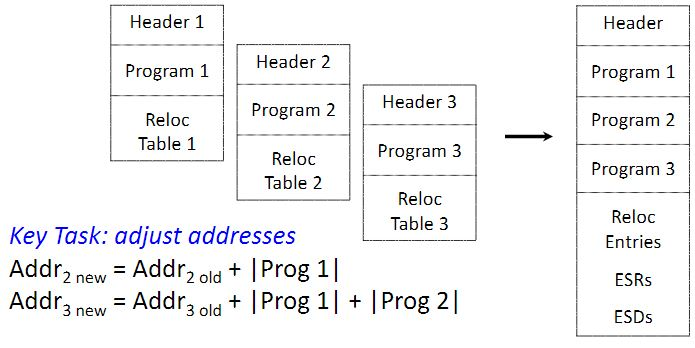
\includegraphics[scale=0.5]{concatenate.JPG}
\end{center}
\caption{Concatenating three files. Courtesy of Prof. Lanctot's slides.}
\end{figure}

\item \textbf{Combine and Adjust ESD's} \\
For the ESD's for program 2, 3, and so on, we must shift them down by the size of all the programs before it (i.e., program 2's ESD must be shifted down by the size of program 1)
\item \textbf{Use new ESD's to update old ESR's} For each old ESR, ff a new ESD exists, update the value at the location $+$ the offset; otherwise adjust the new ESR with the new offset (e.g., ESR$_{\mathrm{2 \,new}} = $ ESR$_{\mathrm{2\,old}} + \vert$Prog 1$\vert$).
\item \textbf{Relocate addresses} Relocate addresses by shifting them based on the offset (e.g., Addr$_{\mathrm{2 \,new}} = $ Addr$_{\mathrm{2\,old}} + \vert$Prog 1$\vert$).
\end{enumerate}
\subsubsection{Dynamic Linking}
What we defined previously is \textit{static linking} (i.e., all of the files are linked before the program is laoded). Another approach is to use \textbf{dynamic linking}, which relocates symbols while a program is running. For instance, if you want to import a new dictionary in Microsoft Word, say one in another language, you would use dynamic linking to load that dictionary file into the running program.
%END%
\end{document}